\documentclass[11pt,letterpaper]{article}
\usepackage[top=3cm, bottom=2cm, left=2cm, right=2cm, columnsep=20pt]{geometry}
\usepackage{pdfpages}
\usepackage{graphicx}
\usepackage{etoolbox}
\apptocmd{\sloppy}{\hbadness 10000\relax}{}{}
% \usepackage[numbers]{natbib}
\usepackage[T1]{fontenc}
\usepackage{ragged2e}
\usepackage[french]{babel}
\usepackage{listings}
\usepackage{color}
\usepackage{soul}
\usepackage[utf8]{inputenc}
\usepackage[export]{adjustbox}
\usepackage{caption}
\usepackage{amsmath}
\usepackage{amssymb}
\usepackage{float}
\usepackage{csquotes}
\usepackage{fancyhdr}
\usepackage{wallpaper}
\usepackage{siunitx}
\usepackage[indent]{parskip}
\usepackage{textcomp}
\usepackage{gensymb}
\usepackage{multirow}
\usepackage[hidelinks]{hyperref}
\usepackage{abstract}
\renewcommand{\abstractnamefont}{\normalfont\bfseries}
\renewcommand{\abstracttextfont}{\normalfont\itshape}
\usepackage{titlesec}
\titleformat{\section}{\large\bfseries}{\thesection}{1em}{}
\titleformat{\subsection}{\normalsize\bfseries}{\thesubsection}{1em}{}
\titleformat{\subsubsection}{\normalsize\bfseries}{\thesubsubsection}{1em}{}

\usepackage{xcolor}
\definecolor{codegreen}{rgb}{0,0.6,0}
\definecolor{codegray}{rgb}{0.5,0.5,0.5}
\definecolor{codepurple}{rgb}{0.58,0,0.82}
\definecolor{backcolour}{rgb}{0.95,0.95,0.92}
\lstdefinestyle{mystyle}{
    backgroundcolor=\color{backcolour},   
    commentstyle=\color{codegreen},
    keywordstyle=\color{magenta},
    numberstyle=\tiny\color{codegray},
    stringstyle=\color{codepurple},
    basicstyle=\ttfamily\footnotesize,
    breakatwhitespace=false,         
    breaklines=true,                 
    captionpos=b,                    
    keepspaces=true,                 
    numbers=left,                    
    numbersep=5pt,                  
    showspaces=false,                
    showstringspaces=false,
    showtabs=false,                  
    tabsize=2
}
\lstset{style=mystyle}

\usepackage[most]{tcolorbox}
\newtcolorbox{note}[1][]{
  enhanced jigsaw,
  borderline west={2pt}{0pt}{black},
  sharp corners,
  boxrule=0pt, 
  fonttitle={\large\bfseries},
  coltitle={black},
  title={Note:\ },
  attach title to upper,
  #1
}

%----------------------------------------------------

\setlength{\parindent}{0pt}
\DeclareCaptionLabelFormat{mycaptionlabel}{#1 #2}
\captionsetup[figure]{labelsep=colon}
\captionsetup{labelformat=mycaptionlabel}
\captionsetup[figure]{name={Figure }}
\newcommand{\inlinecode}{\normalfont\texttt}
\usepackage{enumitem}
\setlist[itemize]{label=\textbullet}

\begin{document}
\begin{titlepage}
\center

\begin{figure}
    \ThisULCornerWallPaper{.4}{Polytechnique_signature-RGB-gauche_FR.png}
\end{figure}
\vspace*{2 cm}

\textsc{\Large \textbf{PHS2223 --} Introduction à l'optique moderne}\\[0.5cm]
\large{\textbf{Équipe : 04}}\\[1.5cm]

\rule{\linewidth}{0.5mm} \\[0.5cm]
\Large{\textbf{Expérience 2}} \\[0.2cm]
\text{Objectif de caméra}\\
\rule{\linewidth}{0.2mm} \\[2.3cm]

\large{\textbf{Présenté à}\\
  Guillaume Sheehy\\
  Esmat Zamani\\[2.5cm]
  \textbf{Par :}\\
  Émile \textbf{Guertin-Picard} (2208363)\\
  Laura-Li \textbf{Gilbert} (2204234)\\
  Tom \textbf{Dessauvages} (2133573)\\[3cm]}

\large{\today\\
Département de Génie Physique\\
Polytechnique Montréal\\}

\end{titlepage}

%----------------------------------------------------

\tableofcontents
\pagenumbering{roman}
\newpage

\pagestyle{fancy}
\setlength{\headheight}{14pt}
\renewcommand{\headrulewidth}{0pt}
\fancyfoot[R]{\thepage}

\pagestyle{fancy}
\fancyhf{}
\renewcommand{\headrulewidth}{1pt}
\fancyhead[L]{\textbf{PHS2223}}
\fancyhead[C]{Objectif de caméra : rapport final}
\fancyhead[R]{\today}
\fancyfoot[R]{\thepage}

\pagenumbering{arabic}
\setcounter{page}{1}

%----------------------------------------------------

\section{Résultats}

Cette section présente et analyse les différentes images capturées lors des
manipulations.

\subsection{Profondeur de champ}

Tout d'abord, les images qui suivent permettent d'analyser la profondeur de champ
du système de lentilles dans deux configurations, soit celle offrant un zoom minimal,
et celle offrant un zoom maximal. Pour obtenir ces images, à chaque extrême de zoom,
le focus est mis sur une cible graduée, à une distance de 1m. Ensuite, cette cible est
déplacée d'abord devant, puis derrière la distance focale, jusqu'à perte du focus.
Cela est déterminé approximativement par la perte de définition entre les graduations
présentes sur la cible. La distance de déplacement jusqu'à cette perte est notée afin
de faire le calcul de profondeur de champ. Pour le zoom minimal :

\begin{figure}[H]
  \centering
  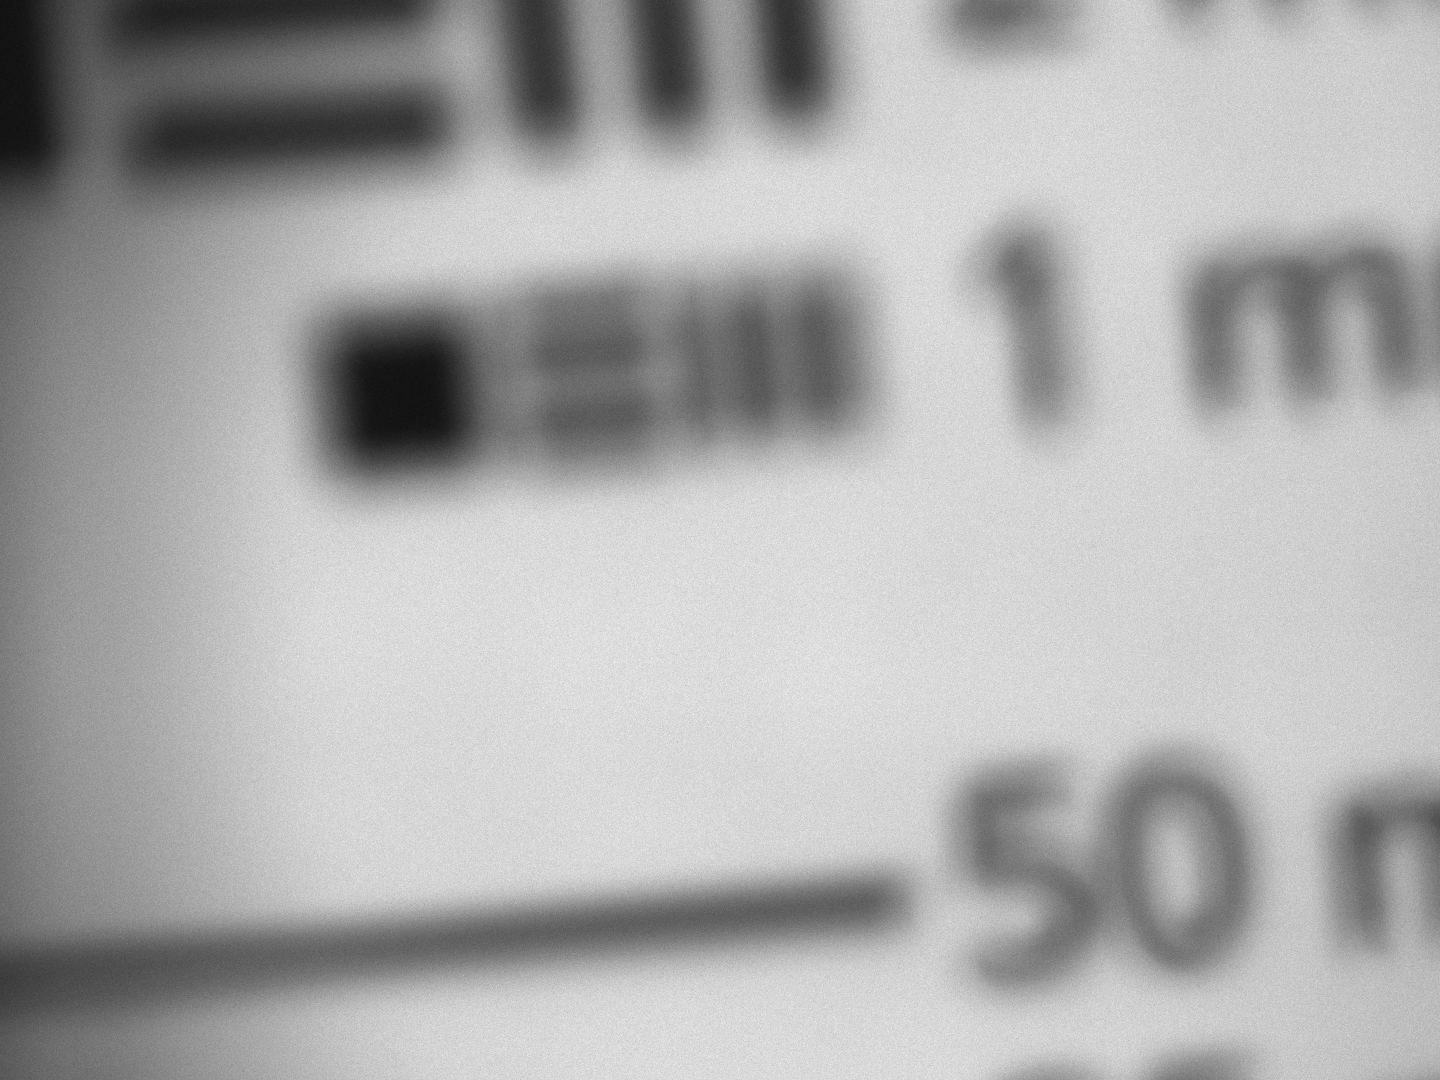
\includegraphics[scale=0.3]{prof_0.458m_min.png}
  \caption{Photo du perte de focus en amont du point focal de 1m, soit à 0.458m,
  pour le zoom minimal.}
  \label{prof_avant_min}
\end{figure}

\begin{figure}[H]
  \centering
  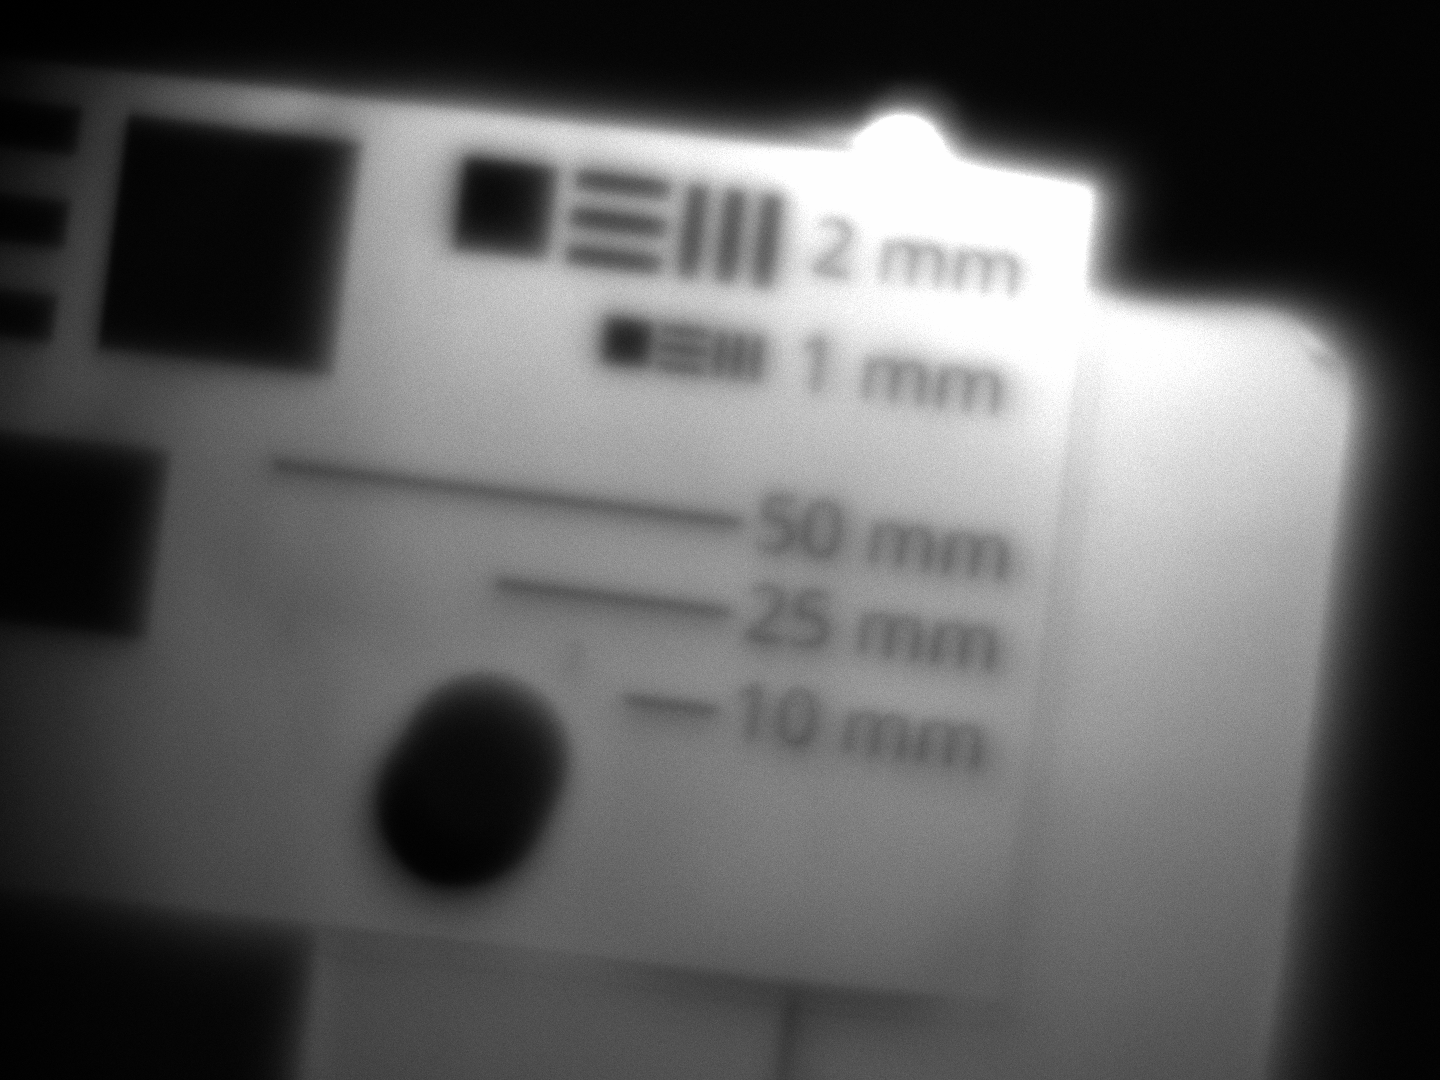
\includegraphics[scale=0.3]{prof_1.986_min.png}
  \caption{Photo du perte de focus en aval du point focal de 1m, soit à 1.986m,
  pour le zoom minimal.}
  \label{prof_arr_min}
\end{figure}

La différence entre les deux positions de perte de focus est donc la profondeur de
champ. Il est donc possible de trouver $\delta_{z,min}= 1.528$m. Pour le zoom maximal :

\begin{figure}[H]
  \centering
  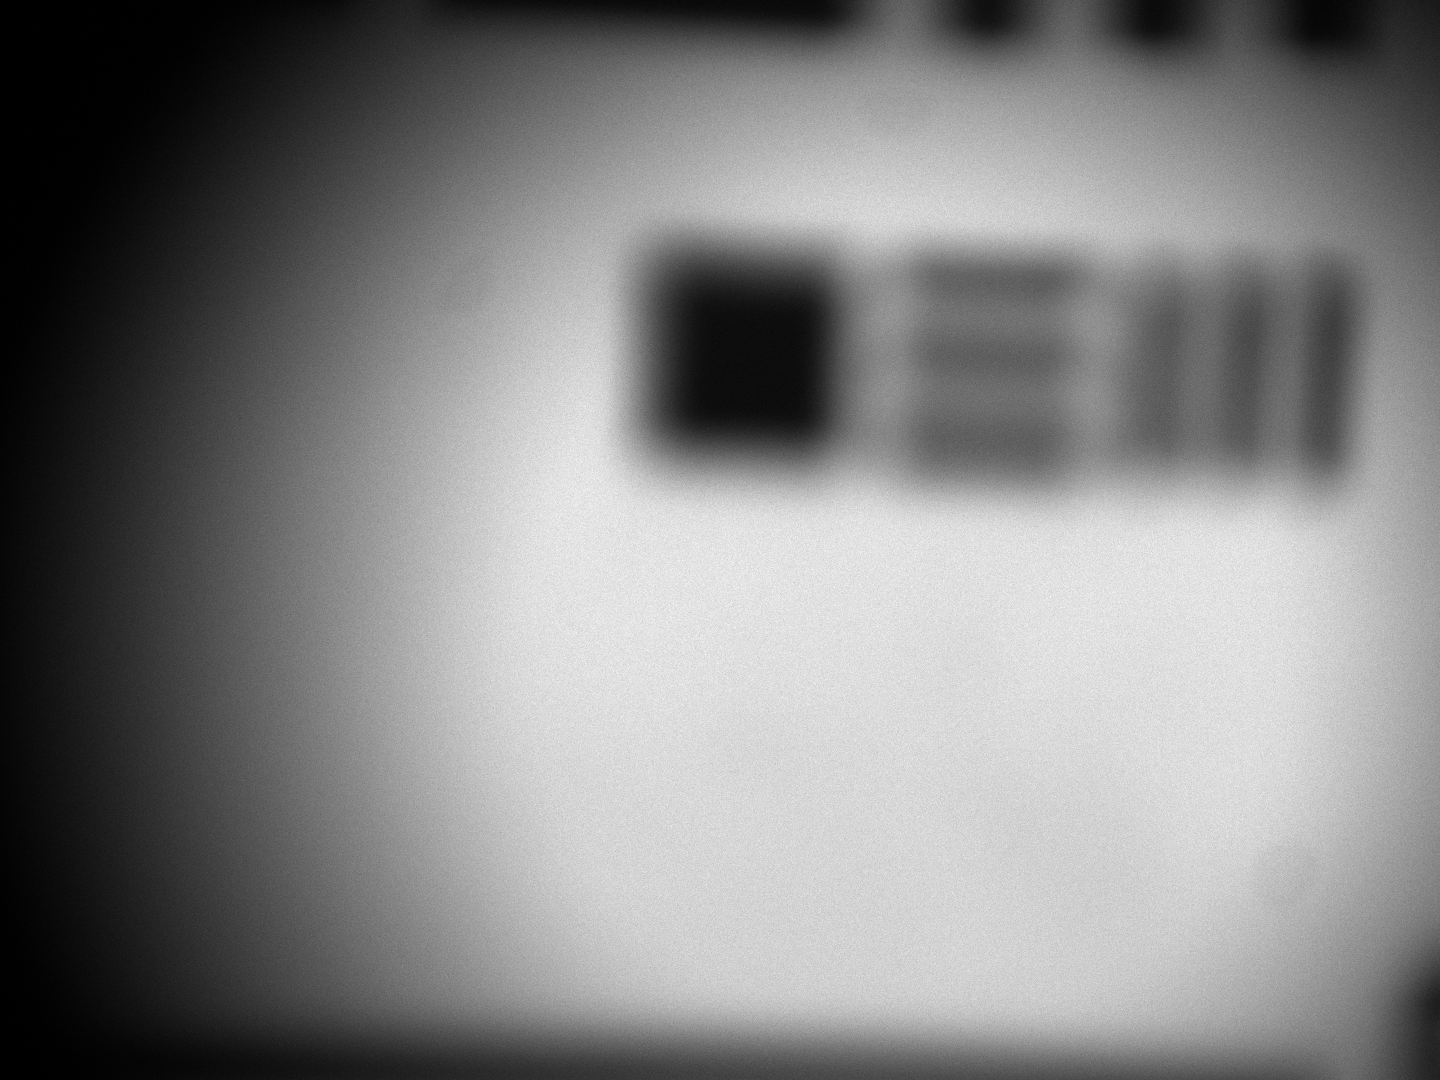
\includegraphics[scale=0.3]{prof_0.711m_max.png}
  \caption{Photo du perte de focus en amont du point focal de 1m, soit à 0.711m,
  pour le zoom maximal.}
  \label{prof_avant_max}
\end{figure}

\begin{figure}[H]
  \centering
  
\includegraphics[scale=0.3]{prof_1.174_max.png}
  \caption{Photo du perte de focus en aval du point focal de 1m, soit à 1.174m,
  pour le zoom maximal.}
  \label{prof_arr_max}
\end{figure}

De la même manière, il est possible de trouver la profondeur de champ 
$\delta_{z,max}= 0.463$m.


\subsection{Analyse de résolution}
 
Afin d'analyser la résolution de la caméra, deux photos de la cible ont été prises
au focus de la caméra à 1m, autant pour le zoom minimal que pour le zoom maximal :

\begin{figure}[H]
  \centering
  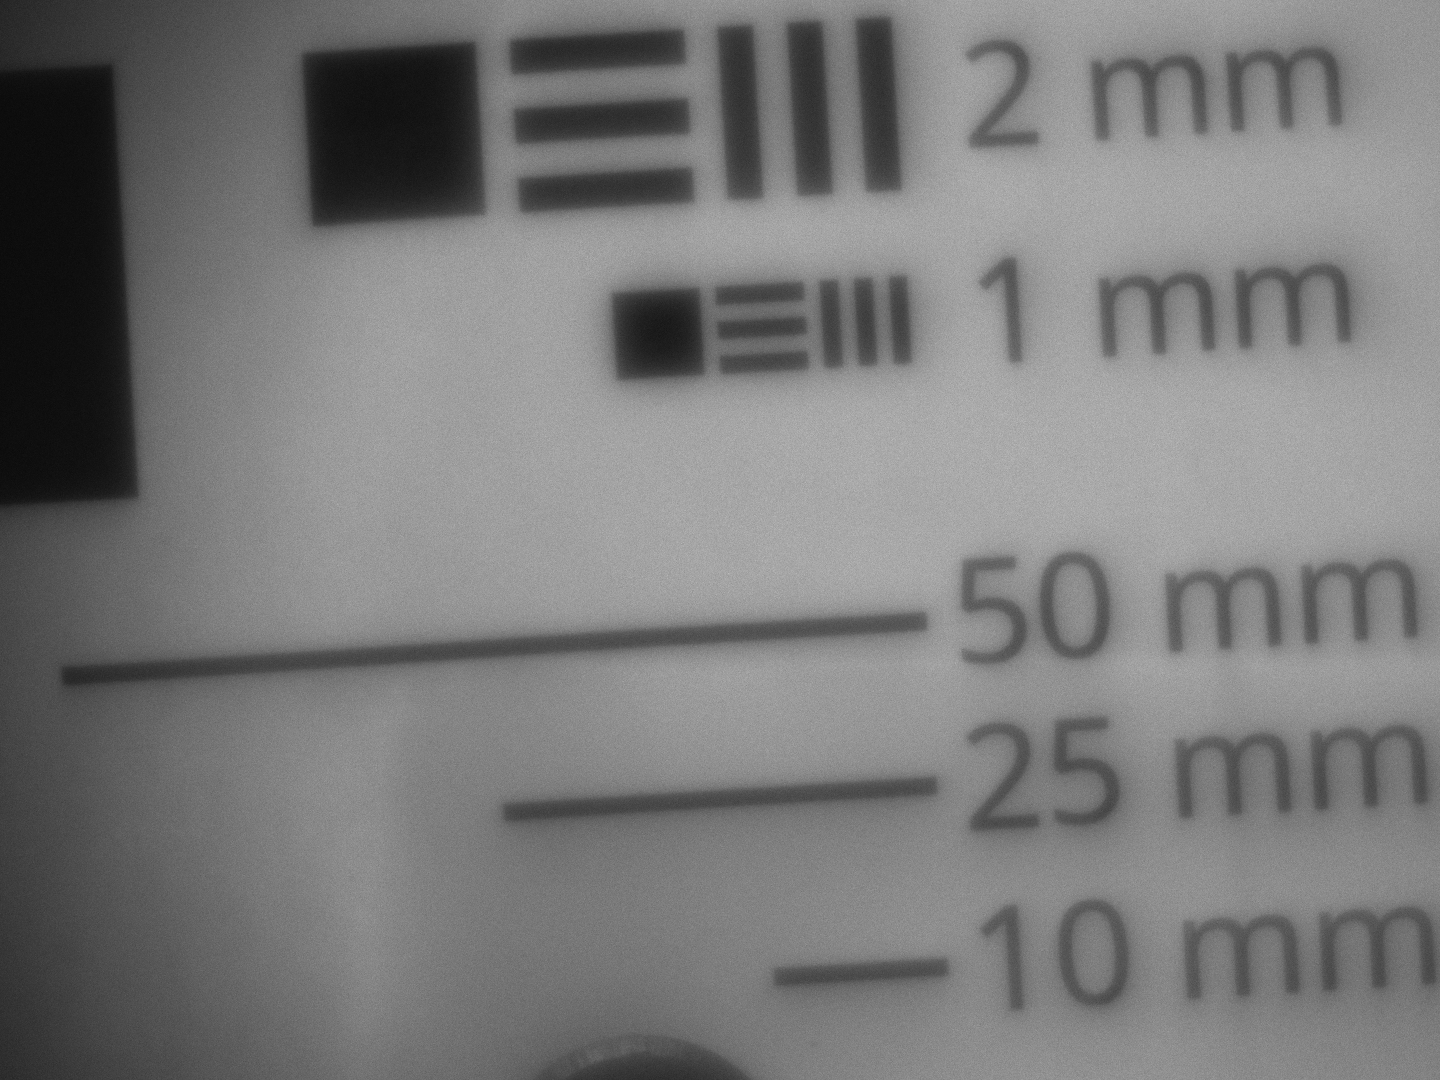
\includegraphics[scale=0.3]{res_1m_min.png}
  \caption{Photo de l'objet au focus de 1m pour le zoom minimal.}
  \label{res_min}
\end{figure}

\begin{figure}[H]
  \centering
  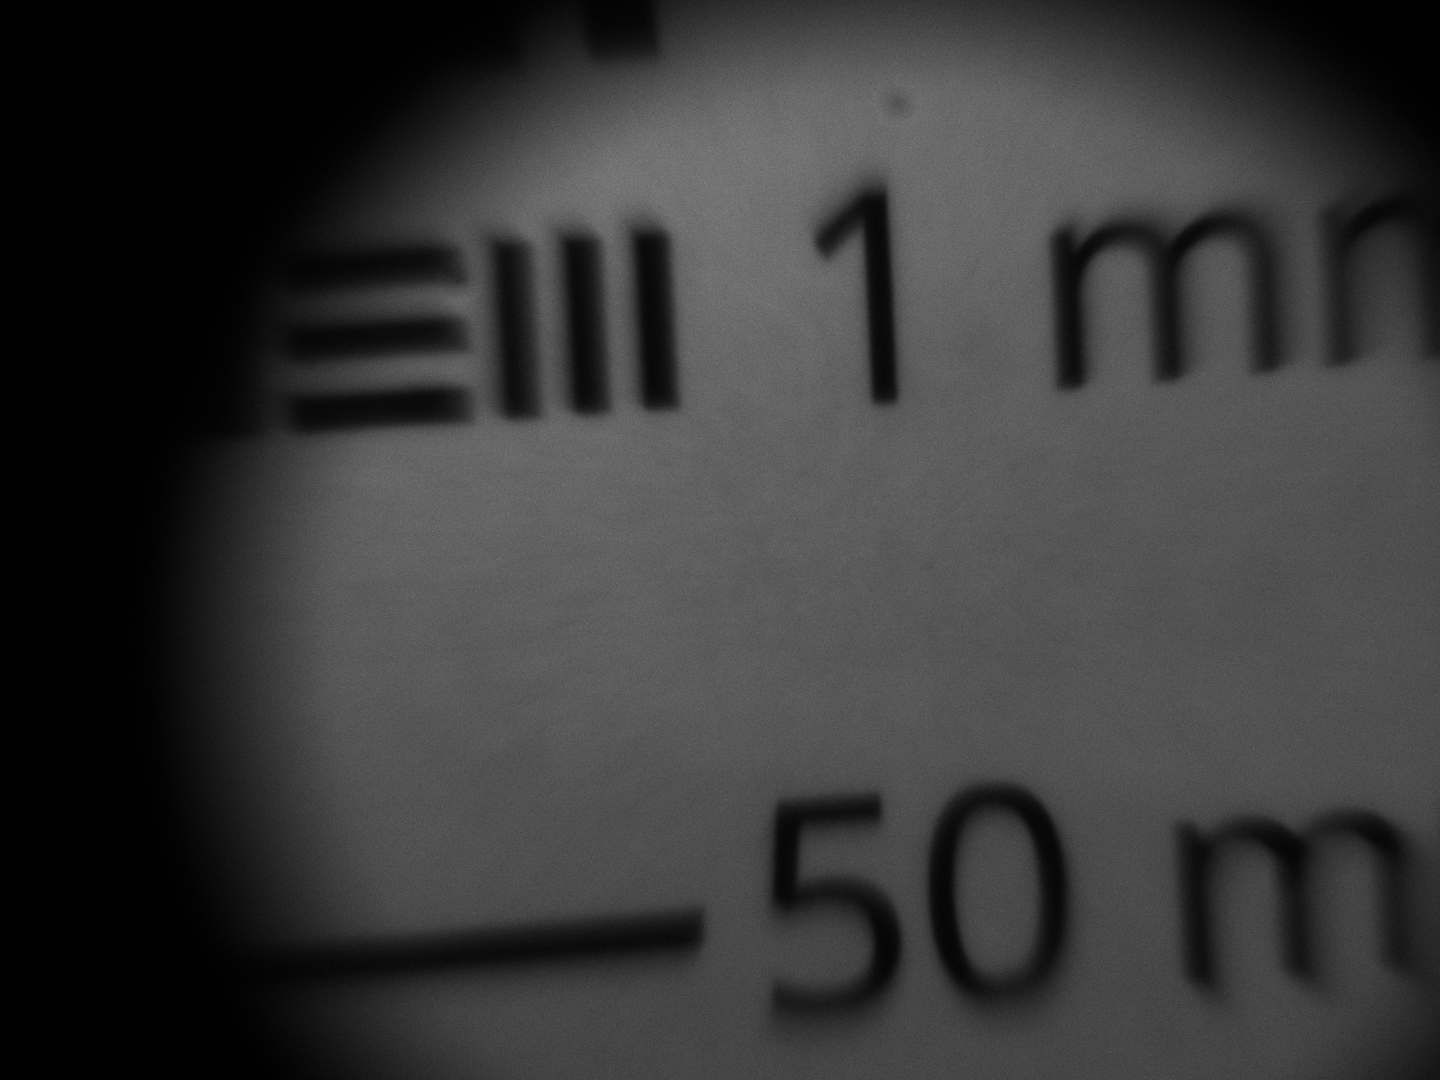
\includegraphics[scale=0.3]{res_1m_max.png}
  \caption{Photo de l'objet au focus de 1m pour le zoom maximal.}
  \label{res_max}
\end{figure}
\textcolor{red}{[TODO Tom]} 


% TODO par Tom : combien de pixels pour les cibles -> taille d'un pixel, 
% analyse d'incertitude (soit donner une incertitude sur les cibles, soit
% faire étude stat sur quelquues mesures de pixels, soit les deux).

% important de décrire le processus et les calculs

\subsection{Vignettage}

L'analyse du vignettage se fait qualitativement en comparant sa présence aux deux
niveaux de zoom, mais aussi à deux positions de l'objet, soit 1m et "l'infini". 
Un vignettage fort est défini par un contour net entre une région circulaire de 
l'image et la région "extérieure" au cercle comme noir. Moins ce contour est net, 
moins le vignettage est fort. Pour l'objet à 1m, en commencant par le zoom minimal : 

\begin{figure}[H]
  \centering
  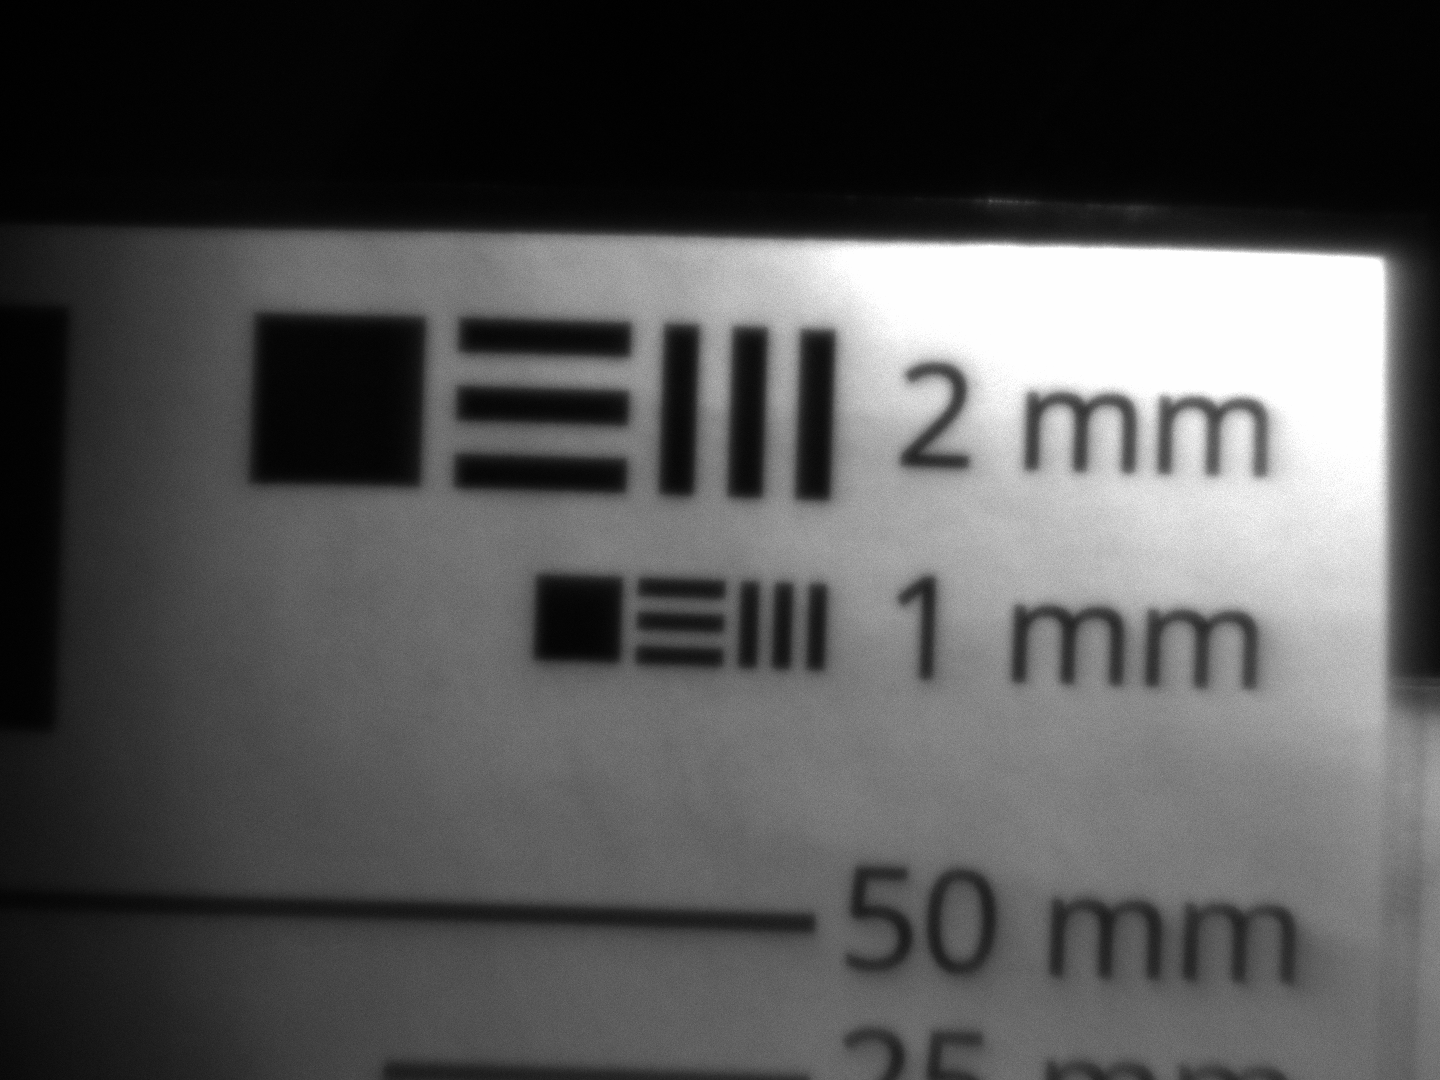
\includegraphics[scale=0.3]{vig_1m_min.png}
  \caption{Image avec vignettage pour un objet à 1m vu avec un zoom minimal.}
  \label{vig_m_min}
\end{figure}

Ce vignettage peut être considéré comme modéré en regardand la région assombrie en 
bas à gauche. Ensuite, avec le zoom maximal :

\begin{figure}[H]
  \centering
  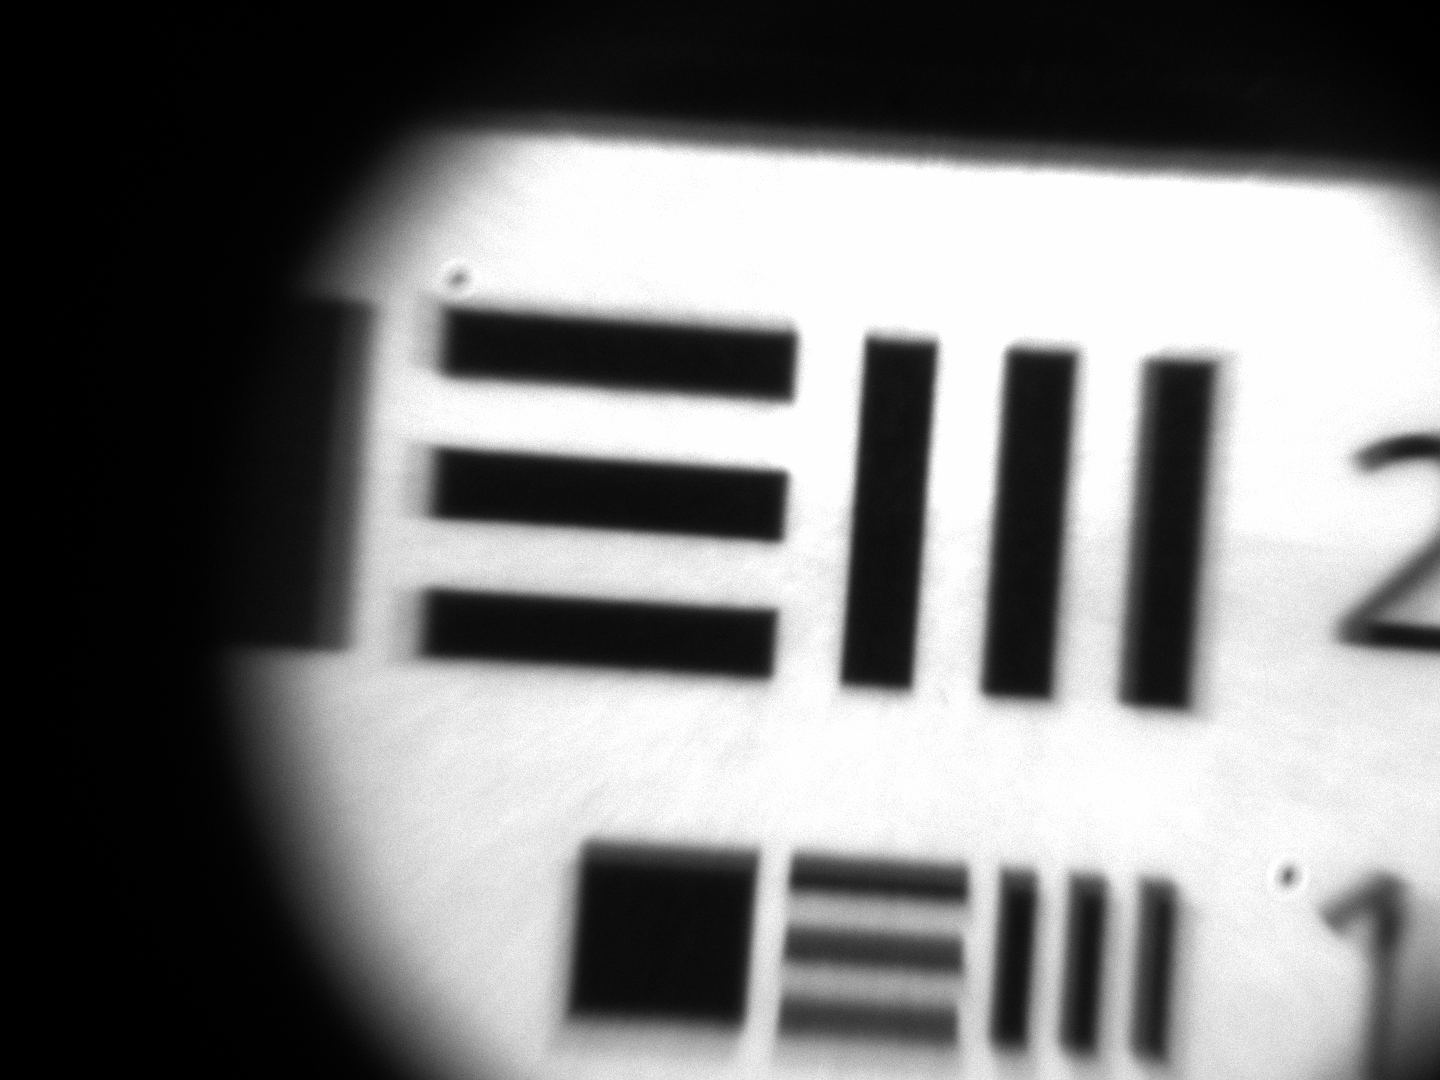
\includegraphics[scale=0.3]{vig_1m_max.png}
  \caption{Image avec vignettage pour un objet à 1m vu avec un zoom maximal.}
  \label{vig_m_max}
\end{figure}

Le vignettage est beaucoup plus important avec ce niveau de zoom, tel que montré par
par la région totalement sombre à gauche. Pour l'objet à l'infini avec le zoom minimal :

\begin{figure}[H]
  \centering
  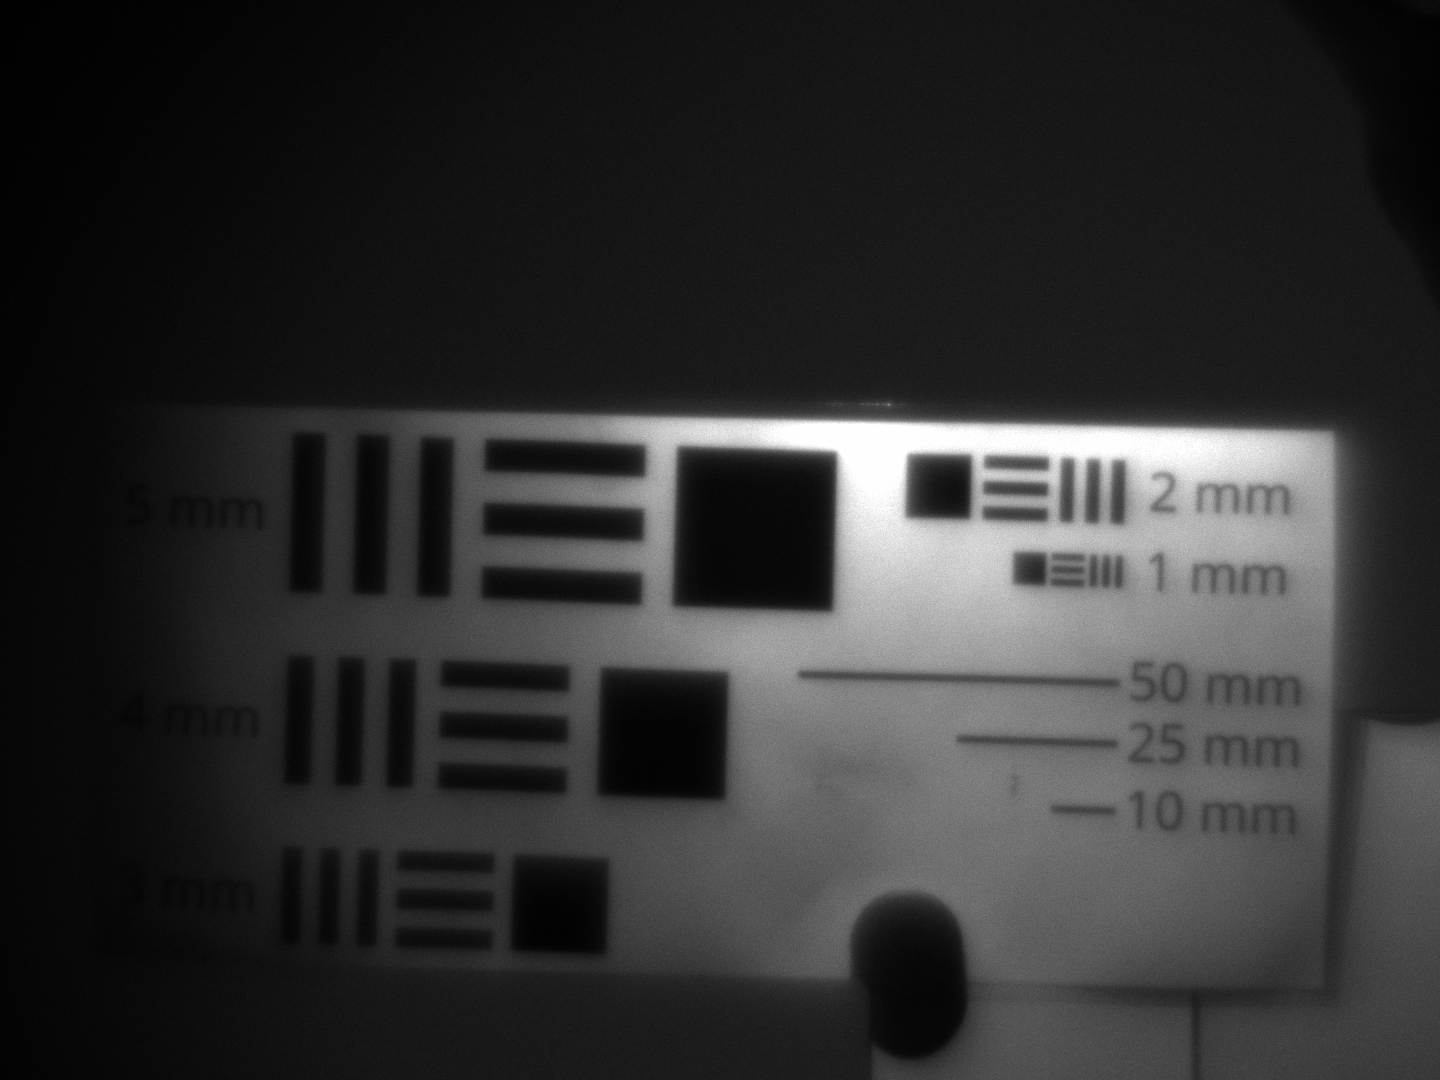
\includegraphics[scale=0.3]{vig_inf_min.png}
  \caption{Image avec vignettage pour un objet à l'infini vu avec un zoom minimal.}
  \label{vig_inf_min}
\end{figure}

Ce vignettage est faible, mais percevable à chaque coin inférieur de l'image. Avec
le zoom maximal :

\begin{figure}[H]
  \centering
  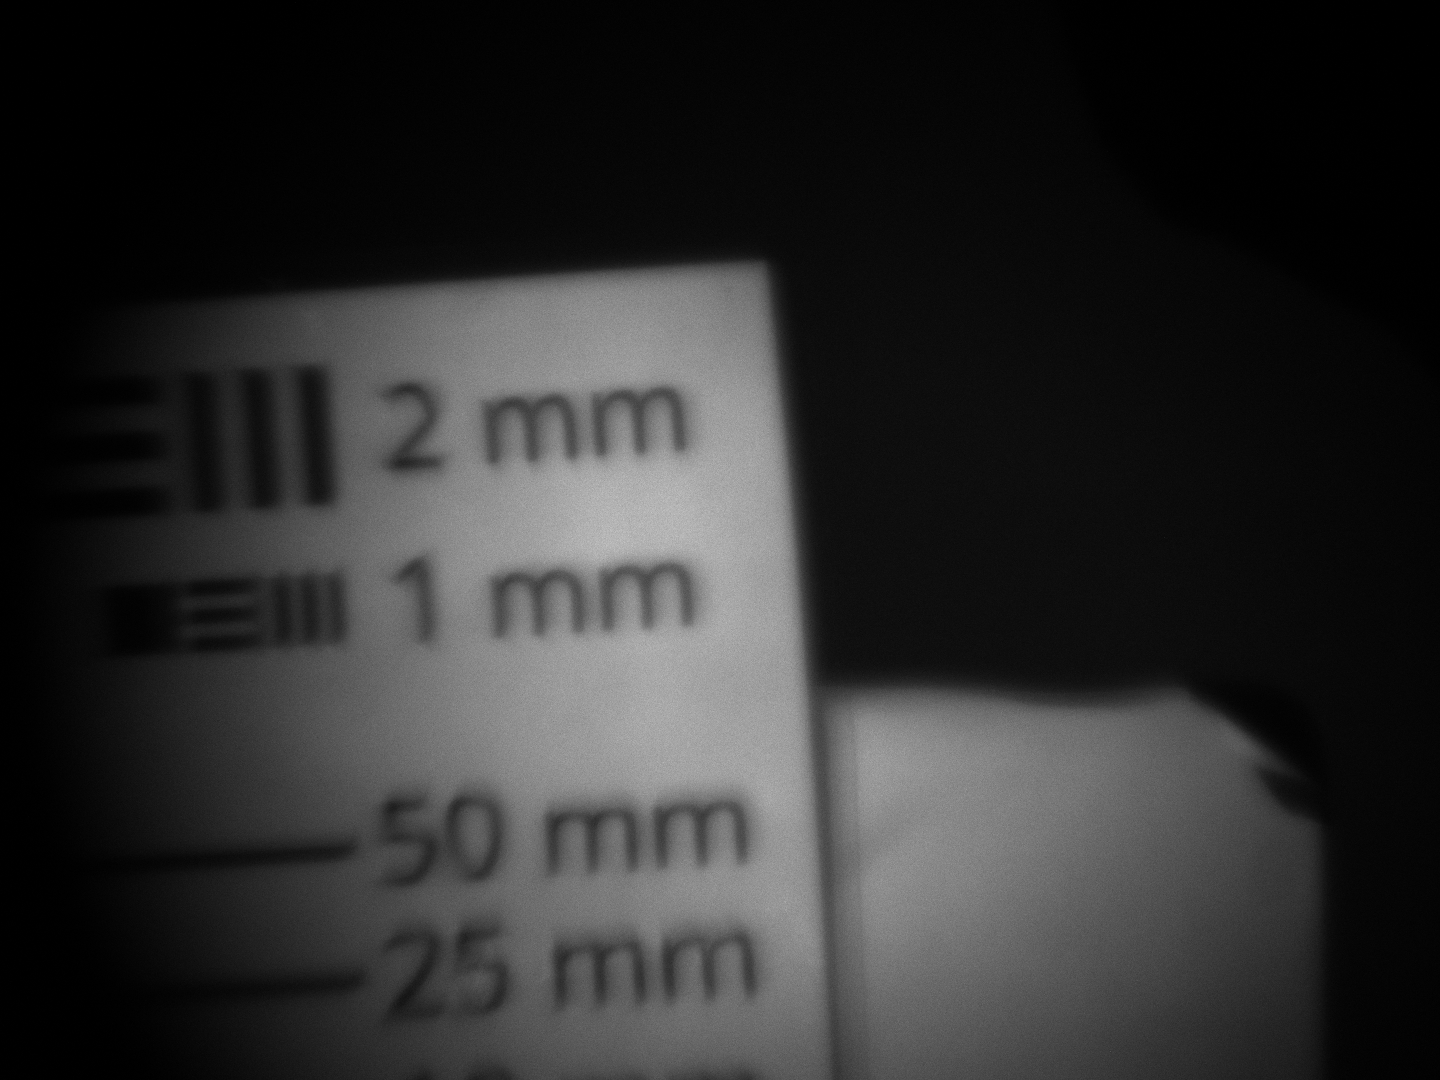
\includegraphics[scale=0.3]{vig_inf_max.png}
  \caption{Image avec vignettage pour un objet à l'infini vu avec un zoom maximal.}
  \label{vig_inf_max}
\end{figure}

Enfin, ce vignettage est aussi modéré, voir fort. On voit une grande région 
assombrie à gauche, mais moins définie qu'à la figure \ref{vig_m_max}.

\subsection{Facteur de zoom}
\textcolor{red}{[TODO Tom]} 
% TODO par Tom : Utiliser les tailles physiques des pixels pour voir la taille de
% la cible a grossi de quel facteur

\subsection{Tableau des caractéristiques}

\begin{table}[h]
\centering
\begin{tabular}{|l|l||l|l|l||c|}
\hline
\textbf{Distance objet} & \textbf{Zoom} & \textbf{Profondeur champ} & \textbf{Résolution} & \textbf{Vignettage} & \textbf{Facteur zoom} \\ \hline
1m & min  & 1.528m & \textcolor{red}{[valeur]} & modéré & \multirow{4}{*}{g} \\ \cline{1-5}
1m & max  & 0.463m & \textcolor{red}{[valeur]} & très fort & \\ \cline{1-5}
Infini & min  & - & \textcolor{red}{[valeur]} & faible & \\ \cline{1-5}
Infini & max  & - & \textcolor{red}{[valeur]} & fort & \\ \hline
\end{tabular}
\caption{Tableau des principaux résultats acquis lors des manipulations.}
\end{table}


\section{Discussion}

Cette section est dédiée à l'analyse, l'interprétation et la critique des résultats
obtenus lors des manipulations.

\subsection{Retour sur l'hypothèse}

Les hypothèses émises précédemment comparaient certaines caractéristiques de performance
de la caméra à la distance entre les lentilles $L_2$ et $L_1$. Cela revient 
essentiellement à analyser les caractéristiques en fonction du zoom. En guise de rappel,
les hypothèses suivantes ont été émises :

\begin{itemize}
\item La profondeur de champ reste constante à environ 6.6mm peu importe le zoom.
\item Plus l'espace entre les lentilles est élevé, plus le zoom est important.
\item Plus l'espace entre les lentilles est élevé, moins la résolution est importante.
\end{itemize}

D'abord, il est très facile de voir que la première hypothèse sur la profondeur
de champ est fausse. Non seulement le comportement n'était pas constant avec le zoom,
mais l'ordre de grandeur est en réalité plus près du mètre que du millimètre. Cette
disparité s'explique facilement par l'omission de l'iris ajustable dans la simulation
faite sur python. Cette dernière peut jouer le rôle d'ouverture d'arrêt, et donc avoir
un impact direct sur la profondeur de champ \textcolor{red}{Source A}. Sans l'avoir 
prise en considération, il est normal que l'hypothèse soit erronée.

% Source A : ndc L8-s5

Ensuite, il est possible de confirmer la deuxième hypothèse sur le zoom. La
configuration avec le zoom maximal utilisé lors de la prise de photo était celle avec
la plus grande séparation entre les lentilles. Le comportement précis de la courbe
trouvée par simulation ne peut être confirmé toutefois, car seulement les deux extrêmes
de zoom ont été testés. Cela implique donc qu'une augmentation de la distance $L_1 - L_2$ implique une augmentation du zoom.

Cette dernière conclusion aide à redéfinir la troisième hypothèse : plus le zoom est
grand, moins la résolution est importante. \textcolor{red}{A FINIR : Emile}.

\subsection{Sources d'erreurs}

\textcolor{red}{TODO: Laura-Li}
éclairage non constant (ouverture et fermeture des lumières)
cible qui bouge quand on était hors de la table
acquisition longue (software qui save pas tout de suite)

\subsection{Réponses aux questions}

\textcolor{red}{TODO : Laura-Li}

\section{Conclusion}

\textcolor{red}{A FAIRE}

\clearpage

% \bibliographystyle{unsrtnat}
% \bibliography{My_Library}

\end{document}
